\chapter{Optical Identification of Variable X-ray Sources}
\label{chap4}

From our lists of matched pairs, we have identified those which potentially exhibit dramatic variability in their X-ray flux. 
This is one half of our goal in this project. 
The other, and arguably more important, half is to determine the source of the X-ray variability.
So naturally, the next step from here is to optically identify our sample of variable X-ray sources in search of AGN.
This is done using the Sloan Digital Sky Survey (SDSS). 
SDSS is an ongoing imaging survey at optical wavelengths using the 2.5 SDSS reflector telescope at the Apache Point Observatory in New Mexico. 
Since 2000, when data collection began, the program has obtained photometric observations for one billion objects and has collected spectra of four million objects. 
To optically identify our targets, we use the SDSS data release 8 (DR8), which was released in January 2011 and covered 14,555 deg$^2$, about 35\% percent of the sky.
We look for spectra and optical images in our list of variable, unique (one-to-one-to-one) matches, in the list of variable ETS sources that had no 2RXS detection but matched to one CSC2.0 source, and the list of multiple match pairs that resulted from Section 3.5.2.
We present first the sources whose X-ray variability could be related to changes in accretion state and then sources whose variability is likely to have a different origin.





\section{Accretion Related X-ray Variability}

%%%%%%%%%%%%%%%%%%%%%%%%%%%%%
%%%%%%%%%%%%%%%%%%%%%%%%%%%%%
%%%%%%%%%%%%%%%%%%%%%%%%%%%%%

\subsection{J122934.1+134630}

J1229+1346, z = 0.099, has 0.5-2.0 X-ray flux values of 4.28$\times 10^{-13}$ \fluxunits, 5.53$\times 10^{-13}$ \fluxunits, and 6.64$\times 10^{-14}$ \fluxunits calculated from the ETS, 2RXS, and CSC2.0, respectively. 
This produces an ETS/2RXS flux ratio of 0.8724, a 2RXS/CSC2.0 flux ratio 7.76, and an ETS/CSC2.0 flux ratio of 8.33. 
Thus, J1229+1346 is considered a highly variable X-ray source from its ETS/CSC2.0 and 2RXS/CSC2.0 flux ratios, which just clear our threshold of 7. 
The SDSS spectrum of the source (Fig 4.1) presents a broad H$\alpha$ emission line with equally dominant [NII] lines on either side of it. 
The strongest line, however, is the narrow [OIII]$\lambda 5007$ line, which completely dominates over the H$\beta$ line to its left. 
These are all indicators which suggest that J1229+1346 is an AGN. 
This is, in fact, the case from BPT diagnostics conducted by \cite{puchnarewicz1992} where J1229+1346 is determined to be a Seyfert 1. 
J1229+1346 is also found in \cite{veron2006}’s extensive catalog of quasars and AGN.

\begin{figure}[t]
    \centering
    \subfloat[]{{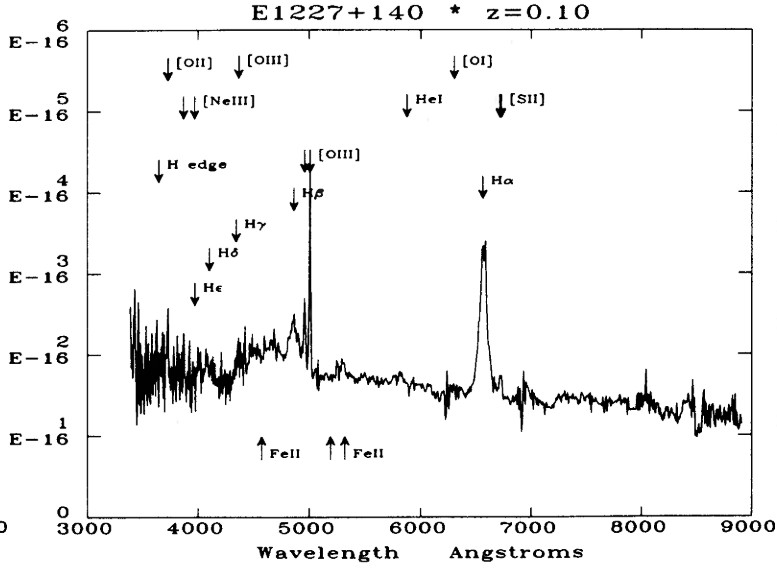
\includegraphics[width=9cm,height=5cm]{spectra/j1229+1346_spectra_paper.jpg} }}%
    \qquad
    \subfloat[]{{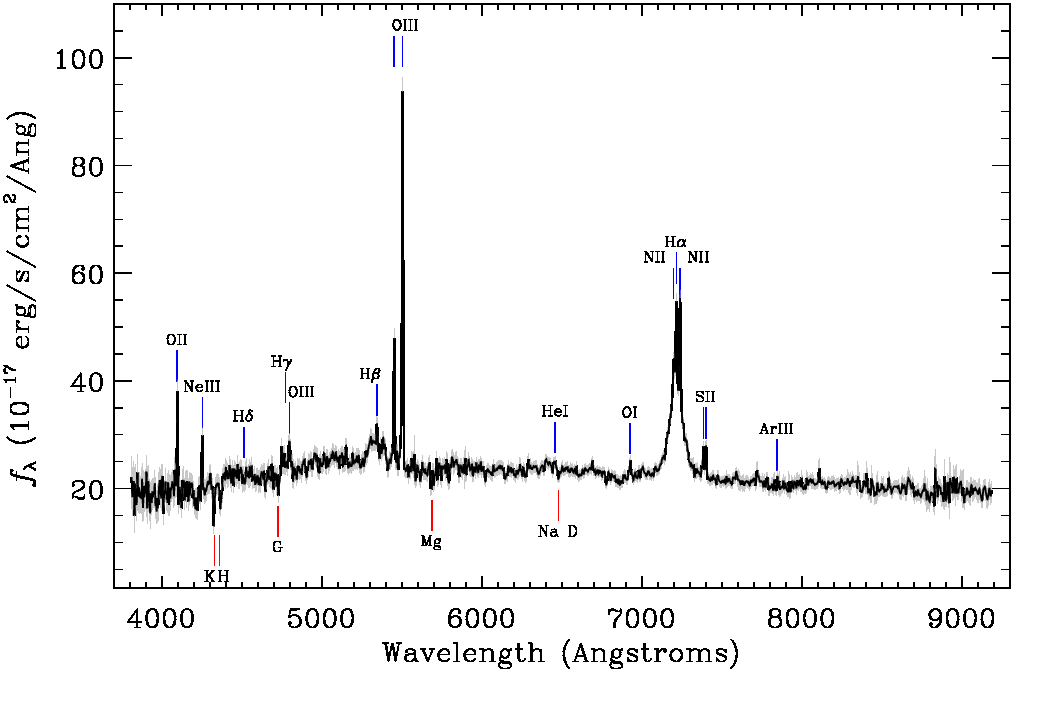
\includegraphics[width=9cm,height=5cm]{spectra/j1229+1346_spectra_sdss.png} }}%
    \caption{The spectra of J1229+1346 taken by \cite{puchnarewicz1992} in 1988 (a) and SDSS in 2005 (b). }%
    \label{fig:example}%
\end{figure}

The literature shows no evidence of some other outstanding physical characteristic which could explain the flux variability in J1229+1346. 
Therefore, it is likely that the observed change in X-ray flux is due to a change in the mass accretion rate of the AGN. 
The fluxes reveal a decrease in the accretion rate from the time of its Einstein and ROSAT observation to its Chandra observation in 2008. 
While the difference in the optical spectra obtained between 1988 and 2005 is minimal, the 1988 spectrum continuum rises to the blue while the SDSS spectrum is level with wavelength. 
This is another indicator of a decrease in activity in the AGN since it could hint at a decrease in the blue power law continuum characteristic of more luminous AGN and quasars. 
In contrast, the continuum in the SDSS spectrum appears to be dominated by starlight from the host galaxy.
The H$\alpha$ and H$\beta$ lines in the 2005 spectrum have relatively the same broadening as the same lines in the 1988 spectrum, so J1229+1346 was and is still a Sey 1.

\FloatBarrier

%%%%%%%%%%%%%%%%%%%%%%%%%%%%%
%%%%%%%%%%%%%%%%%%%%%%%%%%%%%
%%%%%%%%%%%%%%%%%%%%%%%%%%%%%



\subsection{J111520.7+404326}

J1115+4043 has an ETS 0.5-2.0 X-ray flux of 1.43$\times 10^{-12}$ \fluxunits, a 2RXS flux of 1.55$\times 10^{-13}$ \fluxunits, and a CSC2.0 flux of 4.86$\times 10^{-13}$ \fluxunits. 
This results in an ETS/2RXS flux ratio of 9.21, a 2RXS/CSC2.0 flux ratio of 2.94 and an ETS/CSC2.0 flux ratio of 0.313. 
Because of its ETS/2RXS flux ratio, J1115+4043 is considered a variable X-ray source. 
The spectrum from SDSS (shown in Fig 4.2) suggests the source is an AGN due to its broad balmer series lines and strong [OIII] and [NII] lines. 
Obtaining the spectrum and running BPT diagnostics, \cite{akiyama2003} identify the source as a Seyfert 1. 
J1115+4043 is also included in \cite{veron2006}’s catalog of AGN and quasars.


\begin{figure}[h]
    \centering
    \subfloat[]{{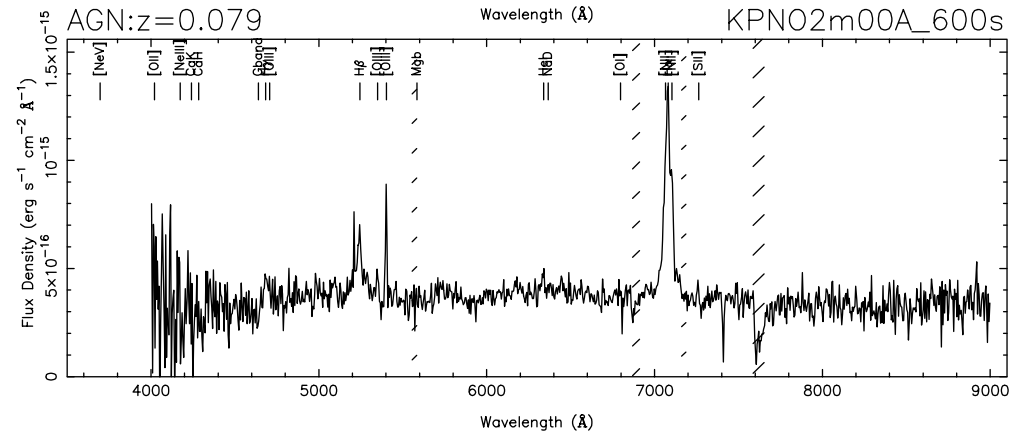
\includegraphics[width=10cm,height=5cm]{spectra/j1115+4043_spectra_paper.png} }}%
    \qquad
    \subfloat[]{{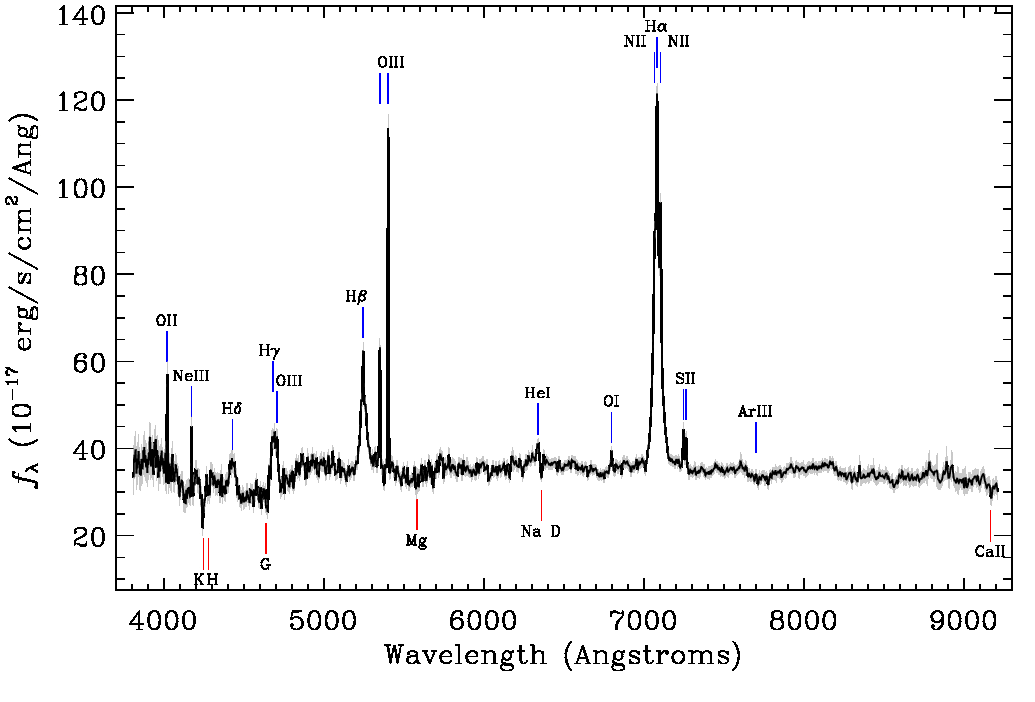
\includegraphics[width=9cm,height=5cm]{spectra/j1115+4043_spectra_sdss.png} }}%
    \caption{The spectra of J1115+4043 taken by \cite{akiyama2003} in 2000-2001 (a) and SDSS in 2003 (b). }%
    \label{fig:example}%
\end{figure}


Because the literature presents no evidence of the X-ray variability being associated with another physical phenomenon in the AGN, we can declare that the variability is likely due to a change in mass accretion rate of the AGN. 
The X-ray flux decreases significantly between the Einstein and ROSAT observations.
It then decreases slightly between the ROSAT observation and the Chandra observation, taken in 2001.
In this case, there is no difference in the optical spectrum, despite the X-ray variability.
This hints at the X-ray variability occurring before the 2000-2001 observation of \cite{akiyama2003}'s spectrum.
Therefore, both spectrum observe J1115+4043 in the same state.


\FloatBarrier
%%%%%%%%%%%%%%%%%%%%%%%%%%%%%
%%%%%%%%%%%%%%%%%%%%%%%%%%%%%
%%%%%%%%%%%%%%%%%%%%%%%%%%%%%




\subsection{J180117.9+662359}

J1801+6623, z = 1.25, has a 0.5-2.0 X-ray flux of 4.32$\times 10^{-13}$ \fluxunits, 1.38$\times 10^{-14}$ \fluxunits, and 1.87$\times 10^{-14}$ \fluxunits observed in the ETS, 2RXS, and CSC2.0, respectively.
This produces an ETS/2RXS flux ratio of 31.4 a 2RXS/CSC2.0 flux ratio of 0.73, and an ETS/CSC2.0 flux ratio of 23.07.
While J1801+6623 does not have a spectrum in SDSS, because it is near the center of the NEP region, a region that has deep exposures in the RASS, extensive information is available from multiple NEP follow up and optical identification projects. 
One of the first identifications of J1801+6623 is in the ROSAT North Ecliptic Pole Deep Survey by \cite{bower1996}. 
Here, J1901+6623 is identified as a quasar. 
It is, again, classified as an AGN in a similar ROSAT North Ecliptic Pole Survey by \cite{henry2006}. 
Both did not make their spectrum available. 
However, we obtain a spectrum of J1801+6623 (show in Fig 4.3) from an observing run at Palomar where we optically followed up on multiple ROSAT sources. 
The spectrum demonstrates a steep power-law spectrum with a broad MgII$\lambda 2800$ line, indicating that J1801+6623 is, in fact, a quasar.

\begin{figure}[h]
\centering
\scalebox{0.65}{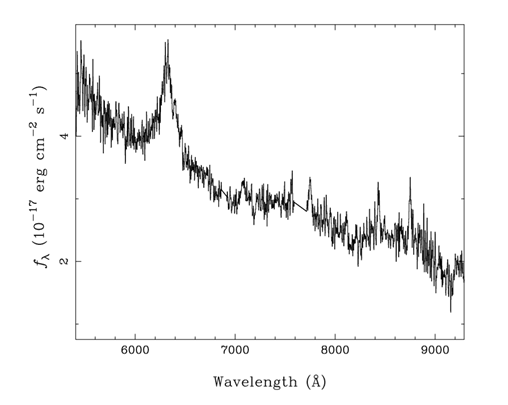
\includegraphics[scale=1]{spectra/j1801+6623_spectra_mdm.png}}
\caption{The spectrum of J801+6623 from Palomar.}
\label{imbeded_fb}
\end{figure}

While J1801+6623 has remained a quasar throughout the different observations, its X-ray flux has not remained consistent. 
Its X-ray flux decreased by a significant amount between the ETS and 2RXS observation.
Since then, it has remained constant between the ROSAT observation and the Chandra observation in 2000.
Its X-ray luminosity has remained above 1$\times 10^{44}$ ergs s$^{-1}$, which agrees with the quasar signatures present in the optical spectrum
The change X-ray flux is likely due to a change in the mass accretion rate of J1801+6623.


\FloatBarrier
%%%%%%%%%%%%%%%%%%%%%%%%%%%%%
%%%%%%%%%%%%%%%%%%%%%%%%%%%%%
%%%%%%%%%%%%%%%%%%%%%%%%%%%%%

\subsection{J082042.4+205715}


J0820+2057, z = 0.114, was not detected in the 2RXS. Ihas an ETS flux of 2.79$\times 10^{-13}$ \fluxunits and a CSC2.0 flux of 2.68$\times 10^{-14}$ \fluxunits in the 0.5-2.0 keV band. 
This produces an ETS/CSC2.0 flux ratio of 10.59, which classifies it as a variable X-ray source.
The SDSS spectrum of J0820+2057 (shown in Fig 4.4) has narrow balmer series lines, showing no initial signs of AGN activity. 
The H$\beta$ and the [OIII] lines appear to be roughly equal strength but the H$\alpha$ and [NII] lines are hard to distinguish. 
For this reason \cite{jackson2012} used the SII/H$\alpha$ line ratio in their BPT diagnostic to reveal that J0820+2057 falls in the category of star forming galaxies. 
However, X-ray observations of J0820+2057 using XMM-Netwon display a high X-ray luminosity (~10$^{43}$ in the 0.3-10 keV bad), which would make it an extremely luminous star-forming galaxy in the X-ray. 
For this reason, \cite{jackson2012} looked for other J0820+2057 physical mechanisms driving this X-ray luminosity. 
They find that J0820+2057 is a compact X-ray source, not extended, and is well fitted by a power law spectrum model, indicating that J0820+2057 is in fact an AGN. 
\cite{jackson2012} infer that the weakened  AGN component in the optical spectrum is a result of enhanced stellar emission.


\begin{figure}[h]
    \centering
    \subfloat[]{{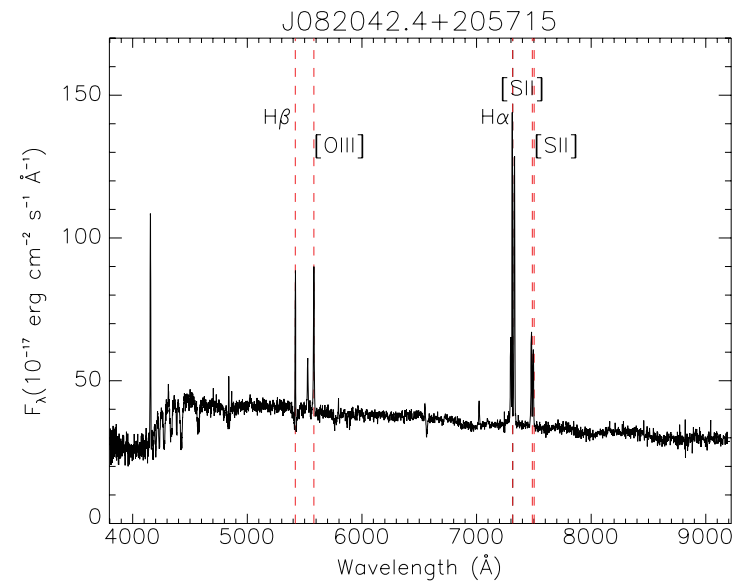
\includegraphics[width=9cm,height=5cm]{spectra/j0820+2057_spectra_paper.png} }}%
    \qquad
    \subfloat[]{{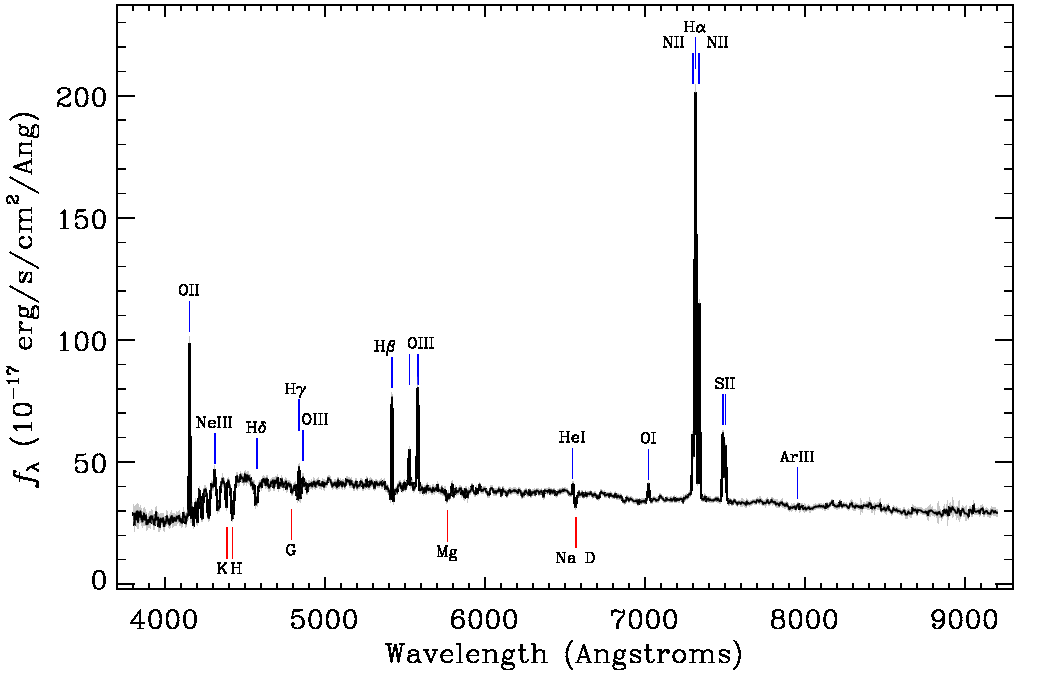
\includegraphics[width=9cm,height=5cm]{spectra/j0820+2057_spectra_sdss.png} }}%
    \caption{The spectra of J0820+2057 taken by \cite{jackson2012} in 2002 (a) and SDSS in 2004 (b). }%
    \label{fig:example}%
\end{figure}


\FloatBarrier

Optically, J0820+2057 is a peculiar source, but it appears that it is a well-behaved X-ray source. 
Thus, its X-ray variability between the ETS and CSC2.0 observations can be attributed to changes in the mass accretion rates of the AGN. 
After its initial observation with Einstein, the X-ray flux dropped significantly before it was observed with Chandra in 2007.


%%%%%%%%%%%%%%%%%%%%%%%%%%%%%
%%%%%%%%%%%%%%%%%%%%%%%%%%%%%
%%%%%%%%%%%%%%%%%%%%%%%%%%%%%

\subsection{J084309.8+292919}

J0843+2929, z = 1.51, was also not detected in the 2RXS. It has an ETS and CSC2.0 X-ray flux of 2.78$\times 10^{-13}$ \fluxunits and 1.68$\times 10^{-14}$ \fluxunits, respectively, in the 0.5-2.0 keV band. 
This produces an ETS/CSC2.0 flux ratio of 16.5, making it a highly variable X-ray source.
The spectrum for J0843+2929 (shown in fig 4.5) has broad Mg, CII, and CIV emission lines and a blue power law continuum. 
These are features characteristic of a quasar.
J0843+2929 has, in fact, been confirmed as a quasar throughout the literature using spectra and photometric observations \citep{schneider2007,richards2015}.


\begin{figure}[h]
\centering
\scalebox{0.55}{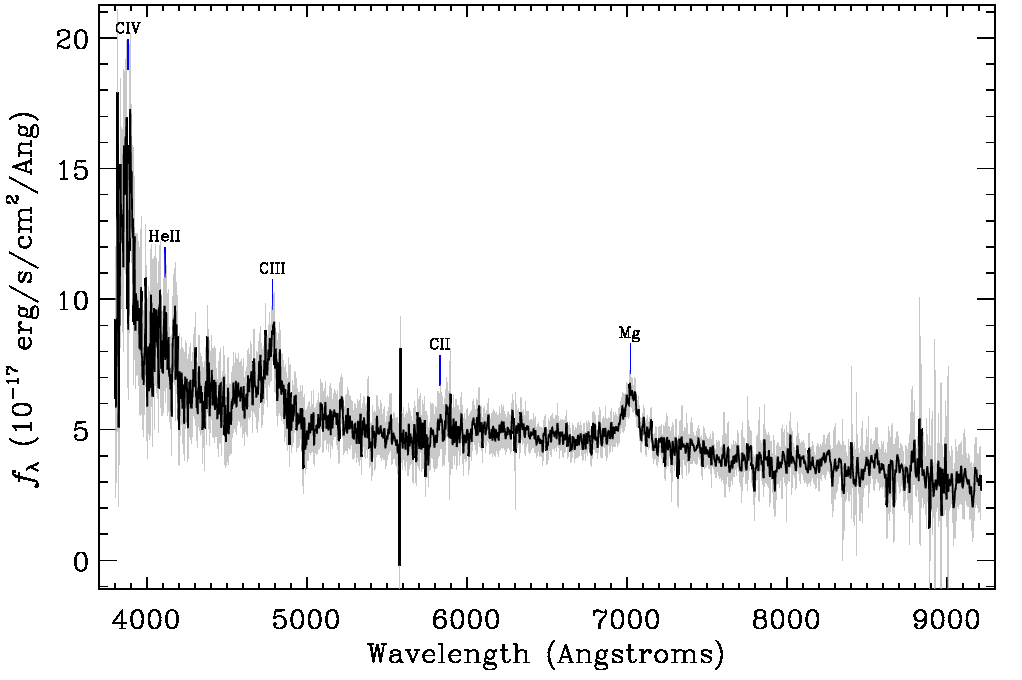
\includegraphics[scale=1]{spectra/j0843+2929_spectra_sdss.png}}
\caption{The spectrum of J0843+2929 taken by SDSS in 2003.}
\label{imbeded_fb}
\end{figure}



We find no evidence for the X-ray variability being associated with any particular physical characteristic. 
Therefore, we can link the variability to changes in the mass accretion rate. 
After it was observed with Einstein, its accretion rate decreased by a significant amount before its Chandra observation was taken in 2001.
Despite these dramatic changes, J0843+2929 is still a quasar and radiating at a high X-ray brightness.


\FloatBarrier




%%%%%%%%%%%%%%%%%%%%%%%%%%%%%%%%%%%
%%%%%%%%%%%%%%%%%%%%%%%%%%%%%%%%%%%%%
%%%%%%%%%%%%%%%%%%%%%%%%%%%%%%%%%%%%

\subsection{Source Luminosities}

As reported in Section 1.2, Seyfert galaxies have a typical luminosity value below 10$^{44}$ erg s$^{-1}$.
If an AGN has a luminosity higher than this, then it enters the range of luminosities typical to quasars.
Therefore, computing luminosity values for AGN can offer an additional diagnostic of their classification.
Thus, we report such values in table 4.1 for the 5 AGN presented above, where we calculate an X-ray luminosity using all available flux values for each source and distance measurements from NED.


%\begin{landscape}
    \begin{table}[h]
    \centering
    \scalebox{0.92}{
    \begin{tabular}{ccccc}
    \hline
    \hline
               source &        $z$  & L$_{\text{ETS}  }$ (erg s$^{-1}$)&  L$_{2\text{RXS}  }$ (erg s$^{-1}$)   &  L$_{\text{CSC}2.0  }$(erg s$^{-1}$) \\
               
    \hline
    
         J122934.1+134630 &     0.099 &  $1.1\times 10^{43}$ &  $1.3\times 10^{43}$ &  $1.6\times 10^{42}$ \\
        J111520.7+404326 &  0.079 &    $2.1\times 10^{43}$ &        $2.2\times 10^{42}$ &           $7.0\times 10^{42}$ \\
        J180117.9+662359 &  1.25 &     $3.8\times 10^{45}$ &         $1.2\times 10^{44}$ &           $1.6\times 10^{44}$ \\
        J082042.4+205715 &  0.11 &  $8.9\times 10^{42}$ &                  N/A & $8.4\times 10^{41}$ \\
        J084309.8+292919 &  1.51 & $3.9\times 10^{45}$  &                  N/A & $2.4\times 10^{44}$ \\
        \hline
        \hline
    \end{tabular}
    }
    \caption{Luminosity values of AGN with accretion-related variability.}
    \end{table}

%\end{landscape}




We see in Table 4.1 that no source crossed the 10$^{44}$ erg s$^{-1}$ luminosity boundary across its ETS, 2RXS, and CSC2.0 observation.
Thus, no source changed its Seyfert/quasar status.
We can use these luminosity values and the 10$^{44}$ erg s$^{-1}$ Seyfert/quasar boundary to classify J1229+1346, J1115+4043, and J0820+2057 as Seyferts.
This classification is consistent with their optical spectra, which also suggests they are Seyferts. 

We can make an additional additional diagnostic using the fact that narrow-line AGNs have a typical soft X-ray luminosity below $ 10^{43}$ erg s$^{-1}$ \citep{stocke1991}.
With this in mind, we see that J1229+1346 and J1115+4043 are potential CLAGN candidates since they cross this boundary.
Because we have a spectra of J1229+1346 during its $>10^{43}$ and $<10^{43}$ epochs, we can rule it out as a CLAGN candidate since its spectrum did not, in fact, change so much so that it is spectroscopically reclassified.
We would need a spectrum of J1115+4043 during its $>10^{43}$ epoch to truly determine it changed in its spectroscopic classification.

Finally, we see that J1801+6623 and J0843+2929 have luminosities greater than the $10^{44}$ Seyfert/quasar boundary.
This classifies them as quasars, which is consistent with their spectroscopic classification.





\FloatBarrier











%%%%%%%%%%%%%%%%%%%%%%%%%%%%%
%%%%%%%%%%%%%%%%%%%%%%%%%%%%%
%%%%%%%%%%%%%%%%%%%%%%%%%%%%%
%%%%%%%%%%%%%%%%%%%%%%%%%%%%%
%%%%%%%%%%%%%%%%%%%%%%%%%%%%%
%%%%%%%%%%%%%%%%%%%%%%%%%%%%%
%%%%%%%%%%%%%%%%%%%%%%%%%%%%%
%%%%%%%%%%%%%%%%%%%%%%%%%%%%%
%%%%%%%%%%%%%%%%%%%%%%%%%%%%%
%%%%%%%%%%%%%%%%%%%%%%%%%%%%%
%%%%%%%%%%%%%%%%%%%%%%%%%%%%%
%%%%%%%%%%%%%%%%%%%%%%%%%%%%%
%%%%%%%%%%%%%%%%%%%%%%%%%%%%%
%%%%%%%%%%%%%%%%%%%%%%%%%%%%%
%%%%%%%%%%%%%%%%%%%%%%%%%%%%%
%%%%%%%%%%%%%%%%%%%%%%%%%%%%%
%%%%%%%%%%%%%%%%%%%%%%%%%%%%%
%%%%%%%%%%%%%%%%%%%%%%%%%%%%%
%%%%%%%%%%%%%%%%%%%%%%%%%%%%%
%%%%%%%%%%%%%%%%%%%%%%%%%%%%%
%%%%%%%%%%%%%%%%%%%%%%%%%%%%%





\section{Non-Accretion Related X-ray Variability}

In the above section, we presented sources which had an X-ray variability likely related to accretion.
We also find sources in which the variability is not accretion related. 
In AGN, there can be a couple of different reasons for X-ray variability if not accretion related. 
The most common of reasons is due to radio-loud AGN, which characteristically display rapid, large amplitude variability due to relativistic beaming effects.
Types of radio-loud AGN that are subject to these effects are BL Lacertae objects and blazars.
Similarly, narrow-line Seyfert 1s also have a characteristic rapid variability in the X-ray that is not related to accretion.
The variability for these types of sources is a result of Compton scattering in the accretion disk \citep{mallick2018}.
A final way in which AGN can vary is due to variations in the absorption column densities associated with dust lanes or a dense dust torus, which can diminist the soft X-ray radiation coming from the nucleus along the line of sight.

Instrumentation differences can also create spurious X-ray variability in sources which might not have experienced any actual variability.
The most common scenario of this type is when observing galaxy clusters or groups.
The modest resolution afforded by the optics of Einstein and ROSAT did not allow them to resolve the discrete point sources within the cluster and in many cases, the extended emission associated with the cluster in nearly point-like.
Therefore, Einstein and ROSAT observed the cumulative and diffuse emission of the galaxy cluster.
Contrary to this, Chandra's fine resolution allows it to make out the discrete point sources within the galaxy cluster, and the point-source search algorithm employed in the construction of the CSC2.0 overlooks the extended emission.
Therefore, any variability associated with these types of observations is likely due to the different resolving power of the instruments and is likely not real.

Below, we present cases where we found highly variable X-ray emission, but after optically investigating the source, we find galaxies, AGN or other celestial objects that have X-ray variability that is not related to accretion.



\subsection{ J141314.8-031227}


J1413-0312, z = 0.0058, is a well known AGN by the name of NGC5506.
The ETS has a 0.5-2.0 keV flux of 5.55$\times 10^{-12}$ \fluxunits, the 2RXS observes a flux of 7.70$\times 10^{-13}$ \fluxunits, and the CSC2.0 reported a flux of 3.49$\times 10^{-14}$ \fluxunits.
This gives NGC5506 an ETS/2RXS flux ratio of 7.2, a 2RXS/CSC2.0 flux ratio of 22.05, and an ETS/CSC2.0 flux ratio of 158.9.
From all flux ratios, NGC5506 is considered a highly variable source.
It is also clear from the SDSS image and spectrum (show in figure 4.6ab that NGC5506 is a galaxy.
Specifically, it is classified as a Narrow Line Seyfert 1 (NLSy1) by \cite{nagar2002} because of the detection of the permitted OI$\lambda$1.1287$\mu$m line in its spectra (shown in fig 4.6a). 
This line is commonly produced in Seyfert 1s and never in Seyfert 2s.
Additionally, the detection of FeII lines at $\lambda$0.9997$\mu$m, $\lambda$1.0501$\mu$m, $\lambda$1.0863$\mu$m, and $\lambda$1.1126$\mu$m are argued to be produced from BLR clouds and are lines that have only been detected in six other extragalactic objects.
These six objects are also classified as NLSy1s.
NGC5506 also displays another important characteristic which is found in NLSy1s: X-ray variability.
This variability is likely due to the dust lanes found along the galactic disk \citep{nagar2002}.


\begin{figure}[h]
    \centering
    \subfloat[]{{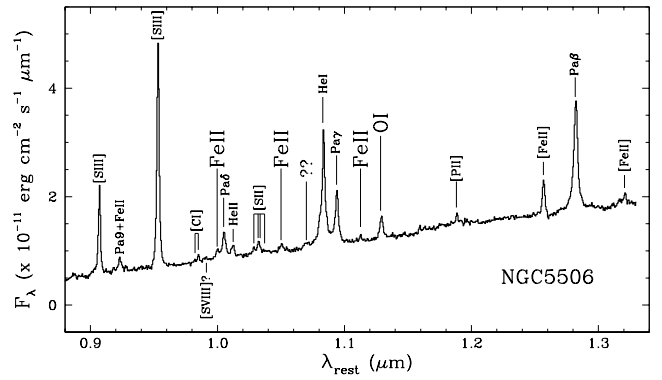
\includegraphics[width=10cm,height=6cm]{spectra/ngc5506_spectra_nagar_paper.png} }}%
    \qquad
    \subfloat[]{{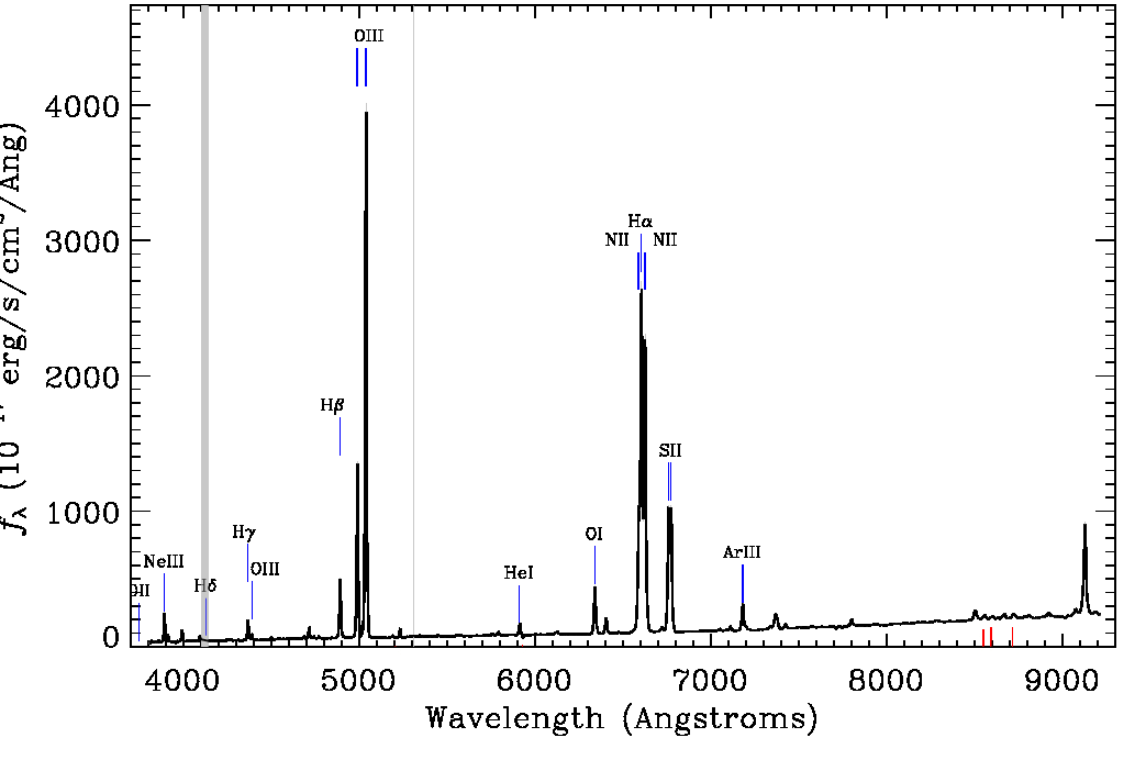
\includegraphics[width=10cm,height=6cm]{spectra/j1413-0312_spectra_sdss.png} }}%
    \caption{The spectrum of NGC5506 taken by \cite{nagar2002} in 2001 (a) and SDSS in 2002. }%
    \label{fig:example}%
\end{figure}





%\begin{figure}[h]
%\centering
%\scalebox{0.55}{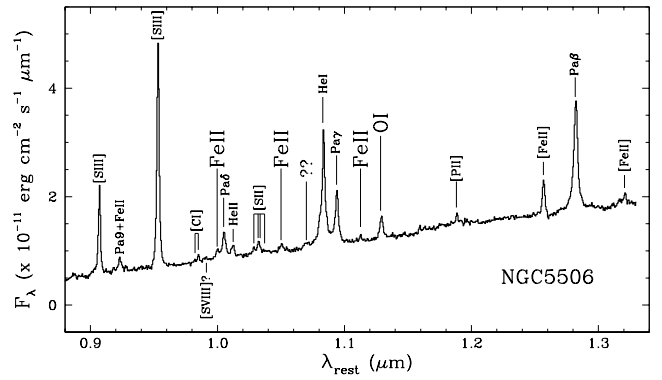
\includegraphics[scale=1]{spectra/ngc5506_spectra_nagar_paper.png}}
%\caption{The spectrum of NGC5506 taken by \cite{nagar2002} in 2001. }
%\label{imbeded_fb}
%\end{figure}

Because NGC5506 has an inclination of 70$^{\circ}$ and is close to being on edge, the dust in the galactic disk causes obscuration of the center, which complicates spectroscopic classifications. 
This has caused NGC5506 to be commonly classified as a type 1.9 or type 2 in the literature. 
This is the case in \cite{garcia2019} where it is classified as a type 1.9 Seyfert. 
In \cite{garcia2019}, NGC5506 is included in their sample of sources used to argue in favor of the AGN unification model. 
In this sample, which includes a total of 24 Seyferts, a torus for each object is modeled based on infrared photometry and spectroscopic measurements. 
Using the National Optical Astronomy Observatory’s (NOAO) CLUMPY, a program that models an AGN’s dust torus and its emission, \cite{garcia2019} derived torus properties for each object in its sample.
For NGC5506,  CLUMPY models the torus to have a bolometric luminosity of $\log(\text{L}_{\text{bol}}) = 43.86$,  a gas mass of 7.6 $\pm_{1.3}^{2.6}$ M$_{\odot}$, an outer radius of 3.8 $\pm_{0.3}^{0.6}$ pc and a torus covering factor of 0.91 $\pm_{0.02}^{0.01}$ \citep{garcia2019}. 
The torus’s bolometric luminosity and its covering factor are evidence for the X-ray variability being due to the dust absorption, as argued by \cite{nagar2002}.
Thus, the X-ray variability can not be directly credited to changes in NGC5506’s mass accretion rate changing.




%%%%%%%%%%%%%%%%%%%%%%%%%%%%%
%%%%%%%%%%%%%%%%%%%%%%%%%%%%%
%%%%%%%%%%%%%%%%%%%%%%%%%%%%%

\subsection{J140621.8+222346}


J1404+2223, z = 0.098, has an ETS 0.5-2.0 keV flux of 1.84$\times 10^{-13}$ \fluxunits, a 2RXS flux of 2.51$\times 10^{-12}$ \fluxunits, and a CSC2.0 flux of 9.17$\times 10^{-13}$ \fluxunits. 
This produces an ETS/2RXS flux ratio of 0.0733, a 2RXS/CSC2.0 ratio of 2.73, and an ETS/CSC2.0 ratio of 0.2. 
It is considered a highly variable X-ray source due to its ETS/2RXS flux ratio. 
J1404+2223 is a well studied source more commonly known as PG1404+226. 
From its SDSS spectra (shown in fig 4.7) and in the literature, PG1404+226 is classified as a NLSy1 \citep{mallick2018}. 
This is due to PG1404+226’s spectrum containing the common properties that define NLSy1s, whose spectra were measured and characterized by \cite{osterbrock1985}. 
The spectrum of PG1401+226 has strong permitted FeII emission lines and has a full width half maximum (FWHM) for H$\beta$ of less than 2,000 km s$^{-1}$. 
The FWHM of H$\beta$ for PG1404+226 is 787 km s${^-1}$ \citep{shangguan2018}.

\begin{figure}[h]
\centering
\scalebox{0.45}{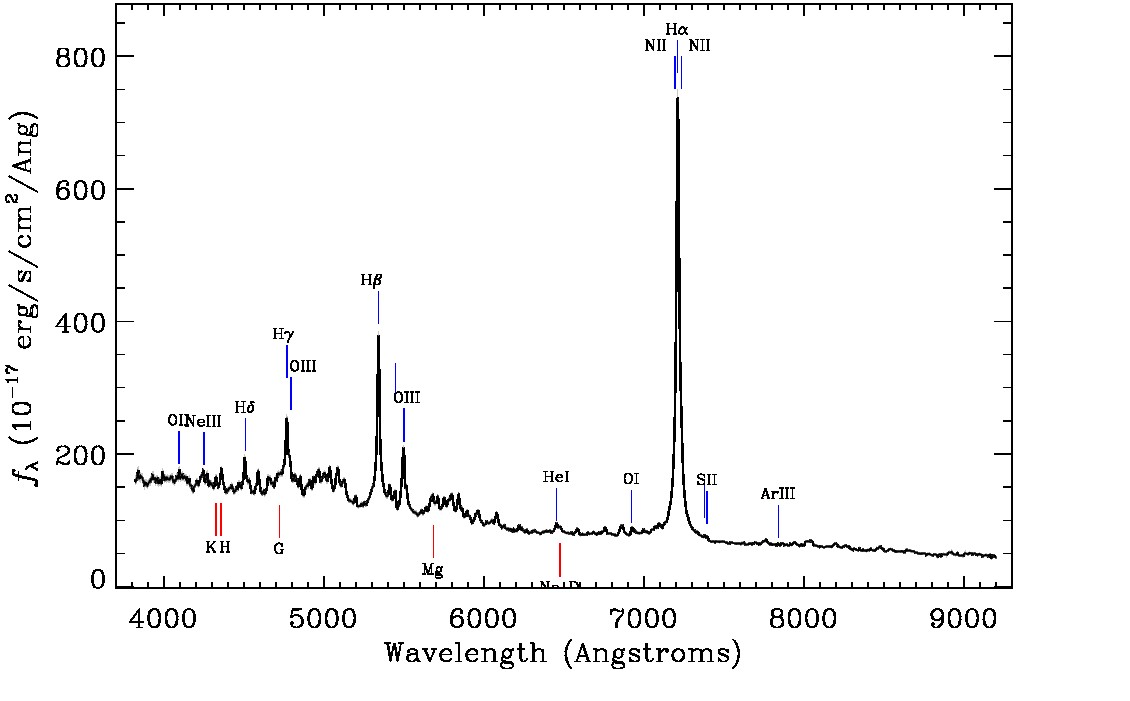
\includegraphics[scale=1]{spectra/j1406+2223_spectra_sdss.jpg}}
\caption{The spectrum of J1406+2223 from SDSS taken in 2008. }
\label{imbeded_fb}
\end{figure}

In \cite{shangguan2018}, the gas content of a sample of quasars are investigated; this sample includes PG1404+226.
Using data from the 2MASS, WISE, and Spitzer telescopes, they construct infrared spectral energy distributions (SEDS) for their sample.
From this, the emission of many physical components of the quasars (stellar, dust torus, dust from the ISM, and of jets for radio-loud quasars) are calculated. 
These properties are used as inputs in the CLUMPY program, which results in best-fit physical measurements.
For PG1404+226, CLUMPY estimates a mass of the dust of $\log(\text{M}_{ \text{d}  }  )$ = 7.89$\pm$ 0.03 M$_{\odot}$ and a mass of gas of $\log(\text{M}_{\text{g}}   )$ 9.99$\pm$0.20 M$_{\odot}$ \citep{shangguan2018}.

As is common in NLSy1s, PG1404+226 experiences large amplitude X-ray variability. 
In \cite{mallick2018}, PG1404+226 is observed to vary in its X-ray flux by a factor of 7 in only 10 ks. 
They hypothesize that this variability is due to variable opacity from the componization of the accretion disk and/or the relativistic reflection of the ionized accretion disk \citep{mallick2018}. 
Thus, the X-ray variability can not be directly credited to changes in PG1404+226’s mass accretion rate changing.

\FloatBarrier

%%%%%%%%%%%%%%%%%%%%%%%%%%%%%
%%%%%%%%%%%%%%%%%%%%%%%%%%%%%
%%%%%%%%%%%%%%%%%%%%%%%%%%%%%

\subsection{J135950.5+623105}

J1359+6231, z = 0.327, has an ETS 0.5-2.0 X-ray flux of 9.52$\times 10^{-13}$  \fluxunits, a 2RXS flux of 6.21$\times 10^{-13}$ \fluxunits and a CSC2.0 flux of 3.4$\times 10^{-14}$ \fluxunits. 
Therefore, it has an ETS/2RXS flux ratio of 1.53, a 2RXS/CSC2.0 flux ratio of 18.26, and an ETS/CSC2.0 flux ratio of 28. 
From its 2RXS/CSC2.0 and ETS/CSC2.0 flux ratios, J1359+6231 is considered a highly variable X-ray source.
Looking at the optical image (shown in fig 4.8) from SDSS makes it clear that this source is, in fact, a galaxy cluster. 

\begin{figure}[h]
\centering
\scalebox{0.60}{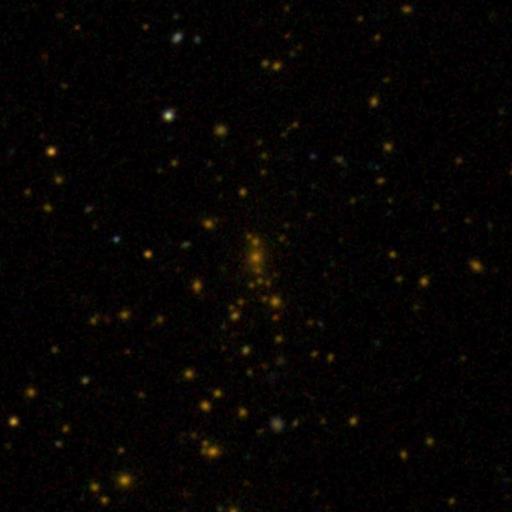
\includegraphics[scale=1]{images/j1359+6231_optical_img_sdss.jpg}}
\caption{The dense optical field around J1359+6231. }
\label{imbeded_fb}
\end{figure}


However, the broad H$\alpha$ line in the spectrum of one of its galaxies  (shown in fig 4.9) suggests that there is a possible AGN within the galaxy cluster. 
For this reason, J1359+6231 has frequently been included in studies which try to distinguish X-ray point sources and/or luminous X-ray galaxies within galaxy clusters. 
\cite{martini2009}, where J1359+6231 is referenced as ZwCl 1358.1+6245, looks for AGN in galaxy clusters to track the evolution of AGN as a function of redshift.
From observations at MDM, \cite{martini2009} find zero AGN with an X-ray luminosity greater than 10$^{43}$ erg s$^{-1}$ within J1359+6231. 
\cite{hart2009} additionally found 67 galaxies in the red sequence and only 1 radio-loud galaxy.

\begin{figure}[h]
\centering
\scalebox{0.60}{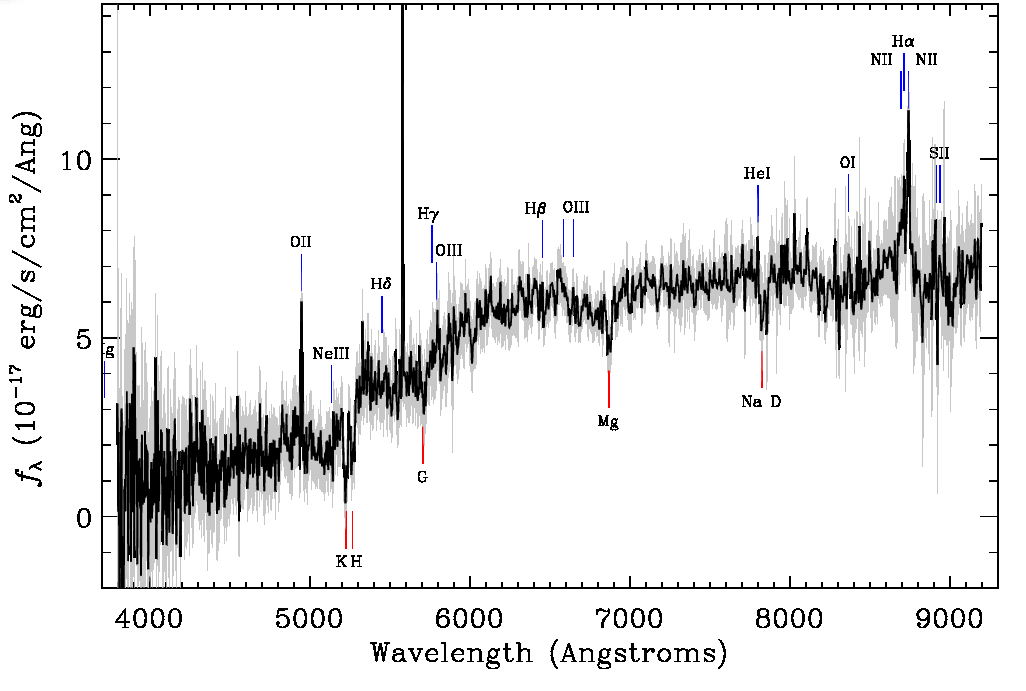
\includegraphics[scale=1]{spectra/j1359+6231_spectra_sdss.png}}
\caption{The spectrum of J1359+6231 taken by SDSS in 2002. }
\label{imbeded_fb}
\end{figure}

There is no evidence for a physical feature being responsible for the variability in the X-ray flux and that is likely because it is not due to a physical feature.
Instead, it is likely that Einstein and ROSAT observed the diffusive emission of the galaxy cluster which must be much greater than the luminosity of the AGN in it while Chandra was able to observe just one of the galaxies from the cluster.
Therefore, the variability can not be attributed to a change in mass accretion rate of a particular AGN.


\FloatBarrier

%%%%%%%%%%%%%%%%%%%%%%%%%%%%%
%%%%%%%%%%%%%%%%%%%%%%%%%%%%%
%%%%%%%%%%%%%%%%%%%%%%%%%%%%%



\subsection{J090720.5+163906}

J0907+1639, z = 0.072,  has an ETS 0.5-2.0 X-ray flux of 5.65$\times 10^{-13}$ \fluxunits, a 2RXS flux of 8.28$\times 10^{-13}$ \fluxunits and a CSC2.0 flux of 2.10$\times 10^{-14}$ \fluxunits. 
This produces an ETS/2RXS flux ratio of 0.682, a 2RXS/CSC2.0 flux ratio of 39.44, and an ETS/CSC2.0 flux ratio of 26.92. 
From its 2RXS/CSC2.0 flux ratio and ETS/CSC2.0 flux ratio, J0907+1639 is considered a highly variable X-ray source. 
The SDSS image and spectrum (shown below in fig 4.10) suggests the source is a regular, elliptical galaxy.
However, upon closer examination, this source is, in fact, a galaxy cluster. 
More specifically, J0907+1639 is classified as a fossil cluster --- a galaxy cluster or group that is dominated by a giant elliptical galaxy at its center \citep{veovodkin2010}. 
Using data from the SDSS-DR13, \cite{omill2019} finds spectroscopic and photometric data for any member of the cluster and determines that J0907+1639 is a low X-ray luminosity galaxy cluster. 
With spectra  collected for 19 members and photometric measurements are found for 32 members, an X-ray luminosity of 0.34$\pm 0.03 \times 10^{44}$ erg s$^{-1}$ is calculated \citep{omill2019}.


\begin{figure}[h]
    \centering
    \subfloat[]{{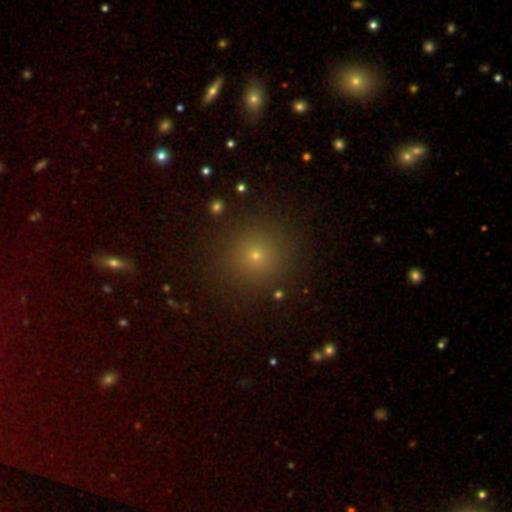
\includegraphics[scale=0.4]{images/j0907+1639_optical_img.jpg} }}%
    \qquad
    \subfloat[]{{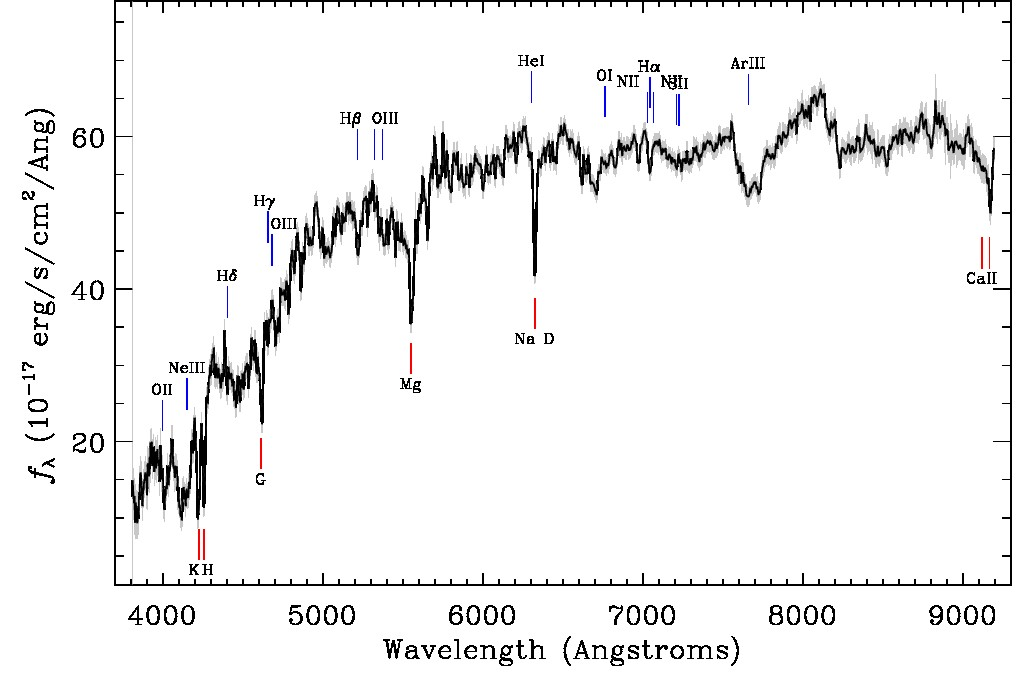
\includegraphics[scale=0.4]{spectra/j0907+1639_spectra_sdss.jpg} }}%
    \caption{The optical field around J0907+1639 showing a dense field of galaxies (a) and J0907+1639's SDSS spectrum (b) taken in 2006 and exhibits no emission-line activity. }%
    \label{fig:example}%
\end{figure}


%\begin{figure}[h]
%\centering
%\scalebox{0.47}{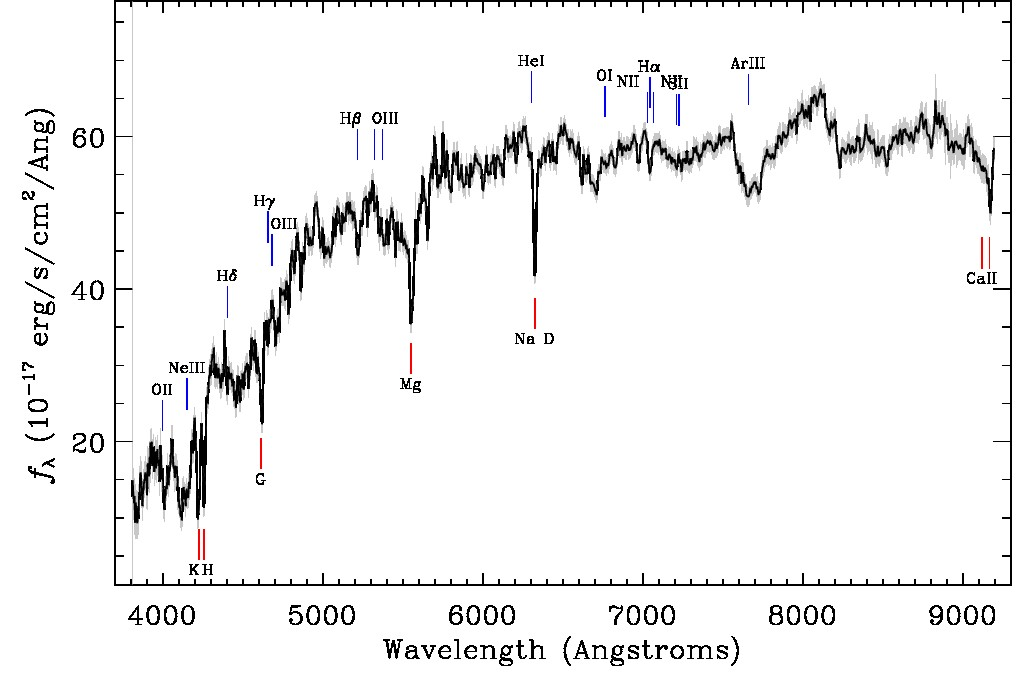
\includegraphics[scale=1]{spectra/j0907+1639_spectra_sdss.jpg%}}
%\caption{The spectrum of J0907+1639 from SDSS. }
%\label{imbeded_fb}
%\end{figure}

No evidence for any physical feature being responsible for the variability in the X-ray flux is found. 
We conclude that the variability is must be spurious. 
Instead, the variability is likely due to the differing optics in the telescopes used. 
That is, Einstein and ROSAT likely observed the diffuse emission of the entire galaxy cluster while Chandra observed only the elliptical at the center. 

\FloatBarrier

%%%%%%%%%%%%%%%%%%%%%%%%%%%%%
%%%%%%%%%%%%%%%%%%%%%%%%%%%%%
%%%%%%%%%%%%%%%%%%%%%%%%%%%%%


\subsection{ J011853.6-010007}



J0118-0100, z = 0.045, is more commonly known as UGC00842. 
It has a 0.5-2.0 X-ray fluxes of 3.92$\times 10^{-13}$ \fluxunits, 2.58$\times 10^{-13}$ \fluxunits, and 1.86$\times 10^{-14}$ \fluxunits calculated from the ETS, 2RXS, and CSC2.0, respectively. 
These values give an ETS/2RXS flux ratio of 1.52, a 2RXS/CSC2.0 flux ratio of 13.88, and an ETS/CSC2.0 flux ratio of 21.09. 
UGC00842 is classified as a highly variable X-ray source due to its 2RXS/CSC2.0 flux ratio and ETS/CSC2.0 flux ratio. 
The SDSS spectrum (shown in fig 4.11) of UGC00842 presents weak emission lines and stellar absorption lines from the stars within the galaxy.
The rather featureless spectrum does not initially suggest the presence of any nuclear activity. 
Radio emission, however, has been detected in UGC00842, which has made it an interesting source to conduct follow up studies on. 
In \cite{brinkmann2000}, which set out to find bright radio and X-ray galaxies by cross correlating the ROSAT All-Sky Survey with the VLA 20cm FIRST Catalog, UGC00842 is found in the cross-correlation and is confirmed to be a BL Lacertae (BL Lac). 
BL Lac are radio-loud AGN characterized by their featureless spectrum with weak emission lines and stellar absorption features, much like spectrum of UGC00842 \citep{falomo2014}.


\begin{figure}[h]
\centering
\scalebox{0.60}{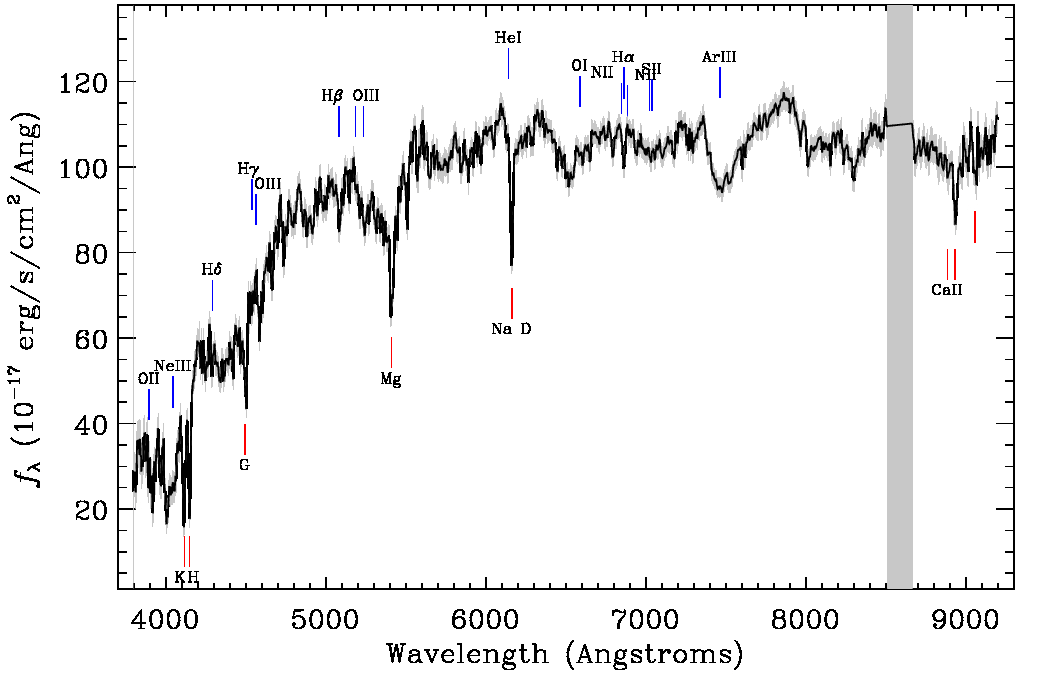
\includegraphics[scale=1]{spectra/j0118-0100_spectra_sdss.png}}
\caption{The spectrum of J0118-0100 taken by SDSS in 2000.}
\label{imbeded_fb}
\end{figure}

Another important characteristic found in BL Lac objects is the large amplitude flux variability present over much of the electromagnetic spectrum. 
In other AGN, X-ray variability can be linked to the accretion rate. 
In BL Lac objects, however, this association can not be made since flux variability is known to be caused by the relativistic beaming of jets stemming from the nucleus.
Therefore, we do not find a change in the accretion rate of UGC00842’s accretion disk.


\FloatBarrier
%%%%%%%%%%%%%%%%%%%%%%%%%%%%%
%%%%%%%%%%%%%%%%%%%%%%%%%%%%%
%%%%%%%%%%%%%%%%%%%%%%%%%%%%%




\subsection{J011515.7+001248}

J0115+0012, z = 0.045, has an ETS 0.5-2.0 X-ray flux of $3.8\times 10^{-13}$ \fluxunits and a CSC2.0 flux of 2.99$\times 10^{-14}$ \fluxunits. 
This produces an ETS/CSC2.0 flux ratio of 12.7, which classifies it as a variable X-ray source. 
The SDSS spectrum for J0115+0012 (shown in fig 4.12 alongside its optical field) suggests it is an AGN due to the broad H$\alpha$ emission line and strong [NII] lines.
The spectrum also displays stellar absorption features. 
While J0115+0012’s spectrum doesn’t hint at any other interesting optical characteristics, J0115+0012 turns out to be a fairly well-studied source, more commonly known as GIN 061. 
GIN 061 was first observed to be the brightest source within galaxy cluster ABELL 0168 \citep{faber1977}. 
Follow up studies on GIN 061 found that it is also a radio-loud galaxy after conducting observations with the JVLA \citep{baldi2015}. 




\begin{figure}[h]
    \centering
    \subfloat[]{{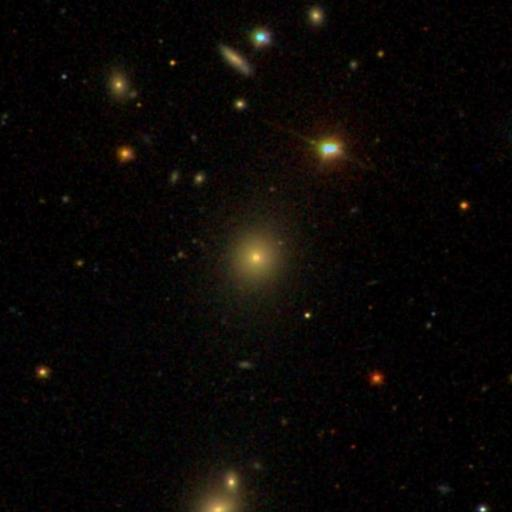
\includegraphics[scale=0.43]{images/j0115+0012_optical_img.jpg} }}%
    \qquad
    \subfloat[]{{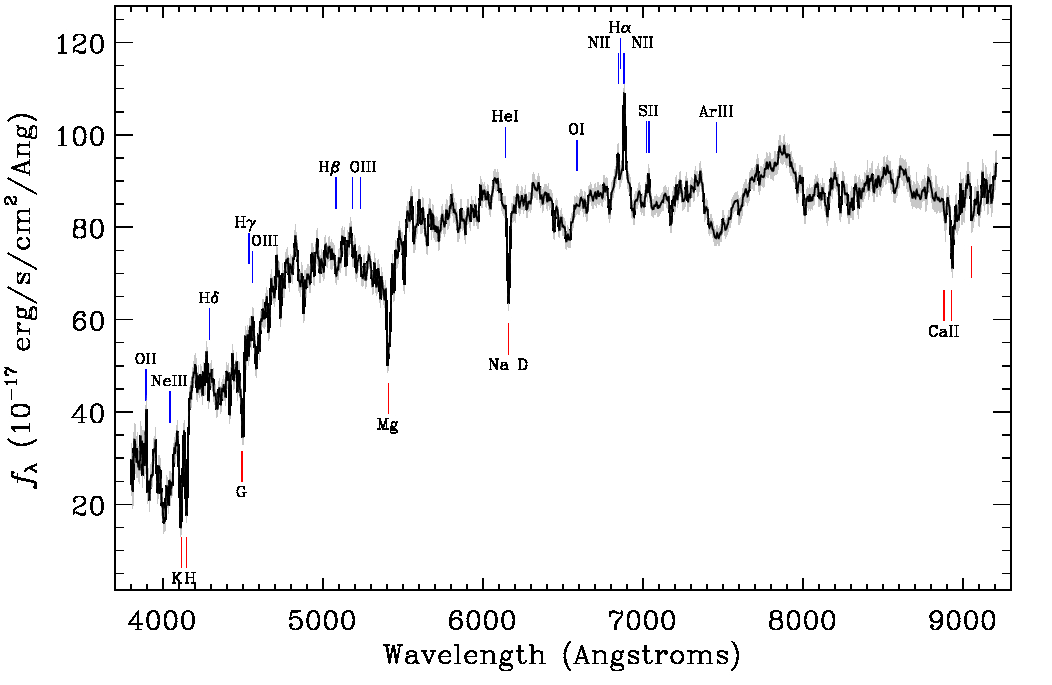
\includegraphics[scale=0.43]{spectra/j0115+0012_spectra_sdss.png} }}%
    \caption{The optical field around J0115+0013 ABELL 0168 (a) and J0907+1639's spectrum taken by SDSS in 2000 (b). }%
    \label{fig:example}%
\end{figure}



%\begin{figure}[h]
%\centering
%\scalebox{0.55}{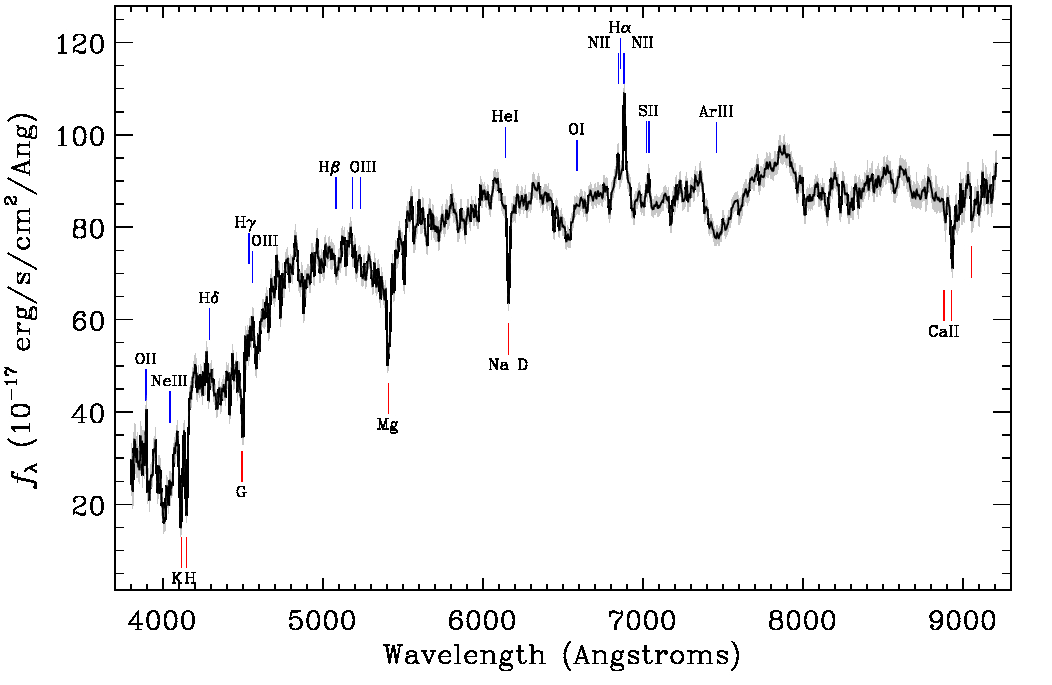
\includegraphics[scale=1]{spectra/j0115+0012_spectra_sdss.png}}
%\caption{The spectrum of J0115+0012 from SDSS.}
%\label{imbeded_fb}
%\end{figure}



\cite{baldi2015} conducted an X-ray study on their 2015 sample of radio galaxies, where GIN 061 and its host cluster were included.
They found that the cluster itself had many sources that are bright in the X-ray in addition to being radio-loud. 
This suggests that the X-ray variability observed is likely an artifact of the telescope optics. 
That is, the Einstein telescope likely observed the diffuse emission of the galaxy cluster as well as the sum of the many X-ray sources confirmed in \cite{baldi2015}.
On the other hand, Chandra’s fine angular resolution allowed it to observe the X-ray emission radiating only from GIN 061. 
For this reason, the variability observed is not due to a change in the mass accretion rate of the source.


\FloatBarrier


%%%%%%%%%%%%%%%%%%%%%%%%%%%%%
%%%%%%%%%%%%%%%%%%%%%%%%%%%%%
%%%%%%%%%%%%%%%%%%%%%%%%%%%%%


\subsection{J132117.8+423515}

J1231+4235, z = 0.79, has an ETS flux of 7.23$\times 10^{-14}$  \fluxunits and CSC2.0 flux of 1.70$\times 10^{-15}$ \fluxunits in the 0.5-2.0 keV band. 
This gives rise to an ETS/CSC2.0 flux ratio of 42.6. 
The SDSS spectrum (fig 4.13) has narrow H$\alpha$ and H$\beta$ emission lines and a strong OIII line. 
Some stellar absorption features are apparent, as well.
With an OIII line much stronger than the H$\beta$ line, J1321+4235 can be classified as an AGN.
J1321+4235 is a well-studied source more commonly known as 3C 285 and long-confirmed as a narrow line AGN \citep{fabiano1984}. 
3C285, however, is also a low excitation radio galaxy (LERG), with a straight jet length of 72 kpc \citep{krause2019}.

\begin{figure}[h]
\centering
\scalebox{0.55}{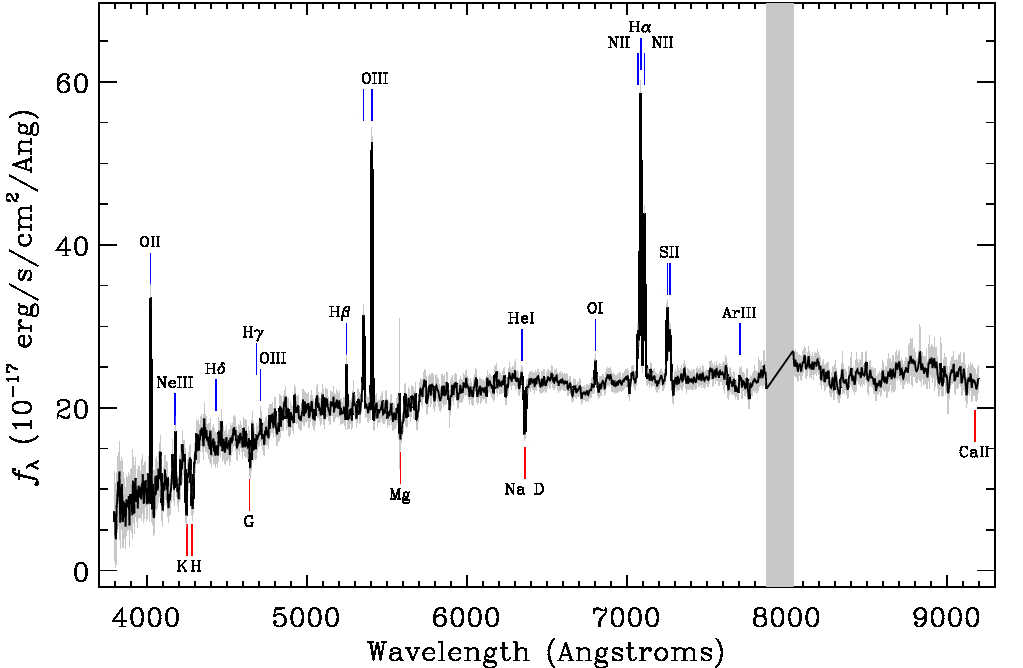
\includegraphics[scale=1]{spectra/j1321+4235_spectra_sdss.png}}
\caption{The spectrum of J1321+4235 from SDSS takn in 2004.}
\label{imbeded_fb}
\end{figure}


A distinctive feature in LERGS is that they have a different kind of accretion mode. 
In standard AGN, cold matter from a disk is accreted onto the SMBH in an efficient fashion.
This mode radiates energy across the electromagnetic spectrum. In LERGS however, accretion is believed to happen in a “hot mode”.
That is, rather than cold matter accreting onto the SMBH, hot gas is being accreted. 
This process is radiatively inefficient and results in little radiated energy, but can produce radio jets, as is the case for 3C285 \citep{best2012}. 
Because of the “hot mode” accretion, no X-ray or IR emission is produced from the accretion \citep{hardcastle2007}. 
Therefore, the X-ray variability in 3C285 is not due to a change in its accretion rate. Rather, because it is a radio source, the variability is likely caused by relativistic beaming effects.

\section{Untangled Multiple Matches}


Following the procedure laid out in Section 3.5.2, we can assess for variability of sources that matched to 2 CSC2.0 sources. Due to our assumptions and the complexity of the scenario, we can have some level or reliability in our findings but must be careful with the interpretation of the variability. Below, we present 1 source that demonstrates high X-ray variability and is found in the SDSS.

\subsection{J083052.2+241056}


J0830+2410, z = 0.938, was one of two CSC2.0 sources that matched a singular 2RXS source. Subtracting the flux of the other CSC2.0 source from the ETS and 2RXS source flux gives values of 3.9$\times 10^{-13}$ \fluxunits and 8.7$\times 10^{-13}$ \fluxunits, respectively. 
The CSC2.0 flux for J0830+2410 is 3.1$\times 10^{-14}$ \fluxunits. 
Therefore, the ETS/2RXS, ETS/CSC2.0, and 2RXS/CSC2.0 flux ratios are 0.44, 28.2, and 12.5, respectively. 
This classified J0830+2410 as a highly variable AGN. From its SDSS spectrum (shown in fig 4.14), it is clear that the source is a quasar. 
The spectrum has a steep power law continuum with broad Mg and H$\gamma$, all which are characteristic of a quasar.
J0830+2410 is in fact, a very well known and well studied source with multiple confirmations of it being a blazar \citep{arsioli2018}. 
These types of sources are known for being radio loud and having relativistic beaming along the line of sight. Blazars are characterized by their flat radio spectrum, which \cite{healey2007} observed J0830+2410 to have.


\begin{figure}[H]
\centering
\scalebox{0.52}{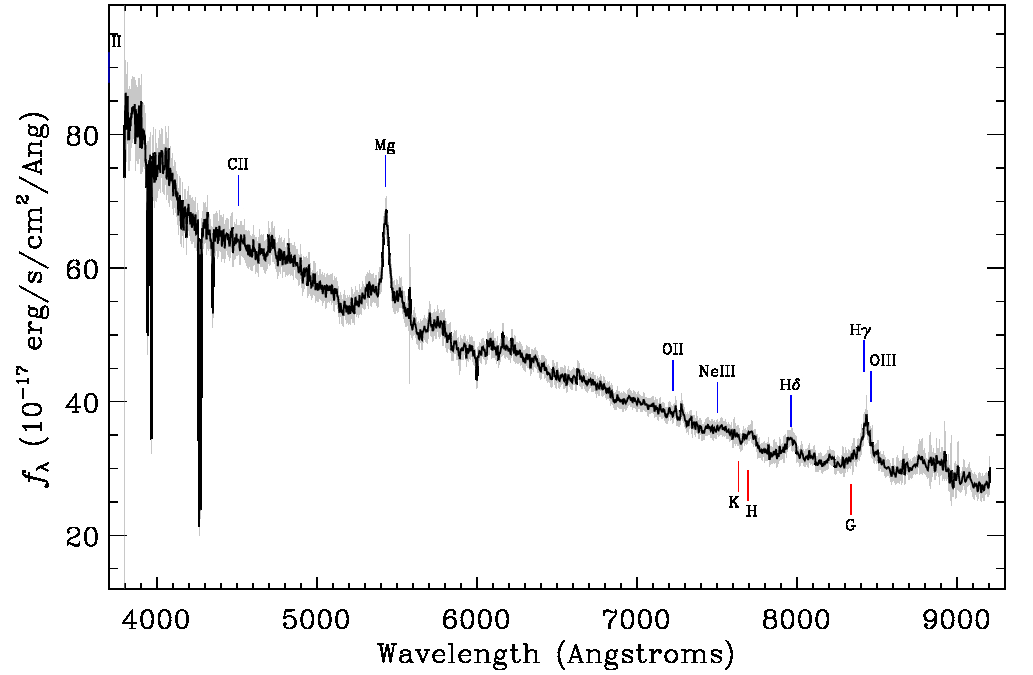
\includegraphics[scale=1]{spectra/j0830+2410_spectra_sdss.png}}
\caption{The spectrum of J0830+3410 taken by SDSS in 2004.}
\label{imbeded_fb}
\end{figure}

Radio sources, and particularly blazars, are known for their high variability, which drowns out much of the thermal radiation from the nucleus. 
Therefore, any X-ray variability that is observed is likely not related to accretion changes. 
Under the assumption that the variability is entirely due to this source and not the other CSC2.0 counterpart that matched to the 2RXS source, the X-ray change can be associated with relativistic beaming effects.


\FloatBarrier